\begin{figure}[tb]
  \centering
  %
  \begin{subfigure}{0.31\linewidth}
  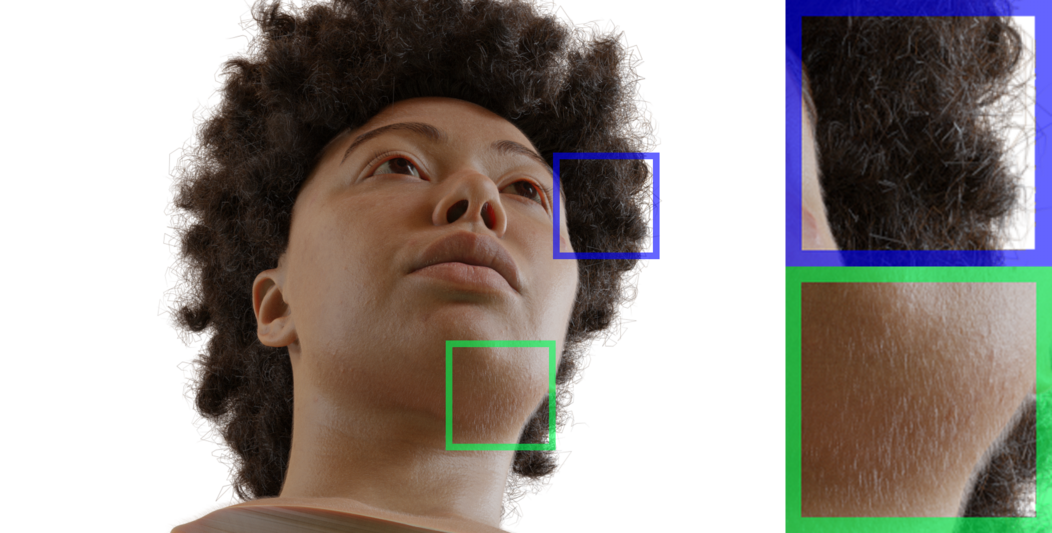
\includegraphics[width=\linewidth]{images/closeup/khady_gt_22_detail.png}
  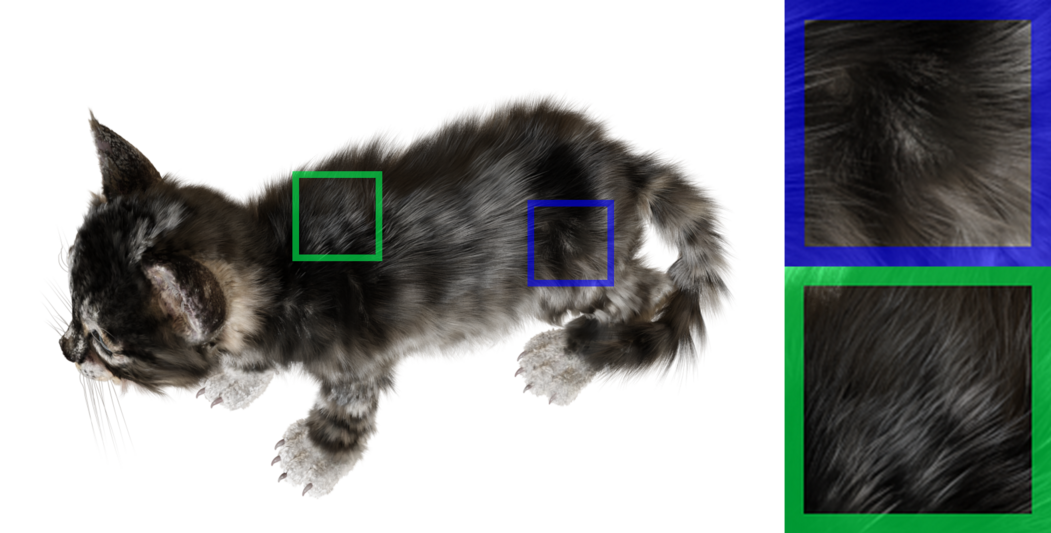
\includegraphics[width=\linewidth]{images/closeup/kitten_gt_67_detail.png}
  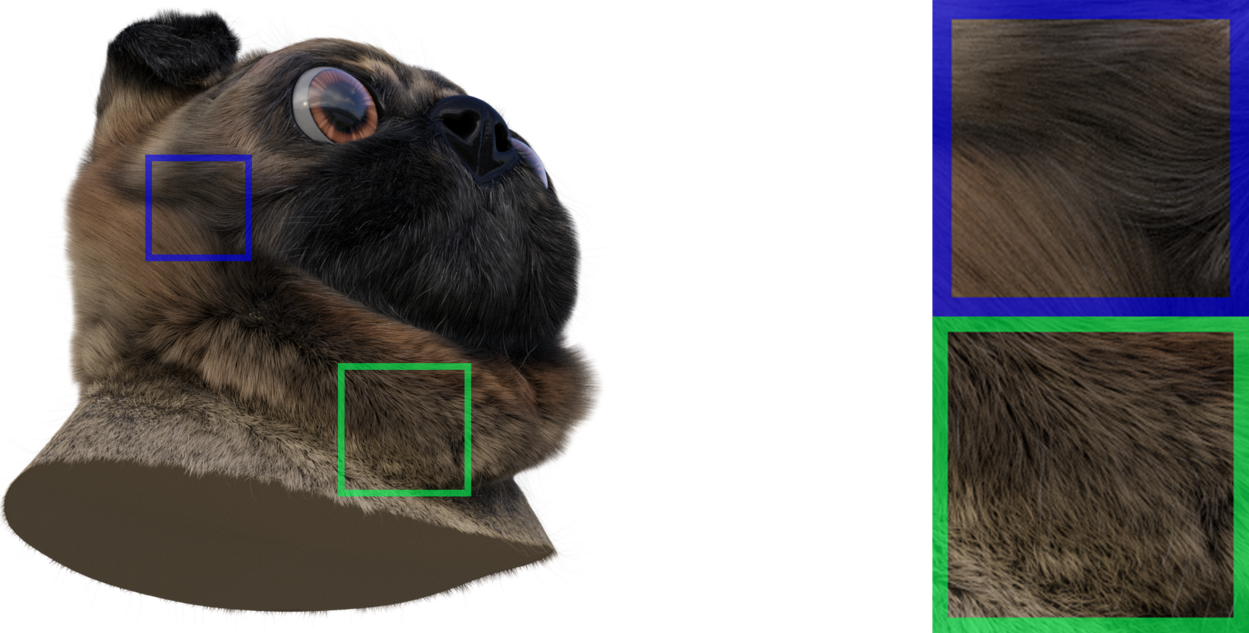
\includegraphics[width=\linewidth]{images/closeup/pug_gt_25_detail.png}
  \caption{Ground Truth Image}
  \end{subfigure}
  %
  \hfill
  %
  \begin{subfigure}{0.31\linewidth}
  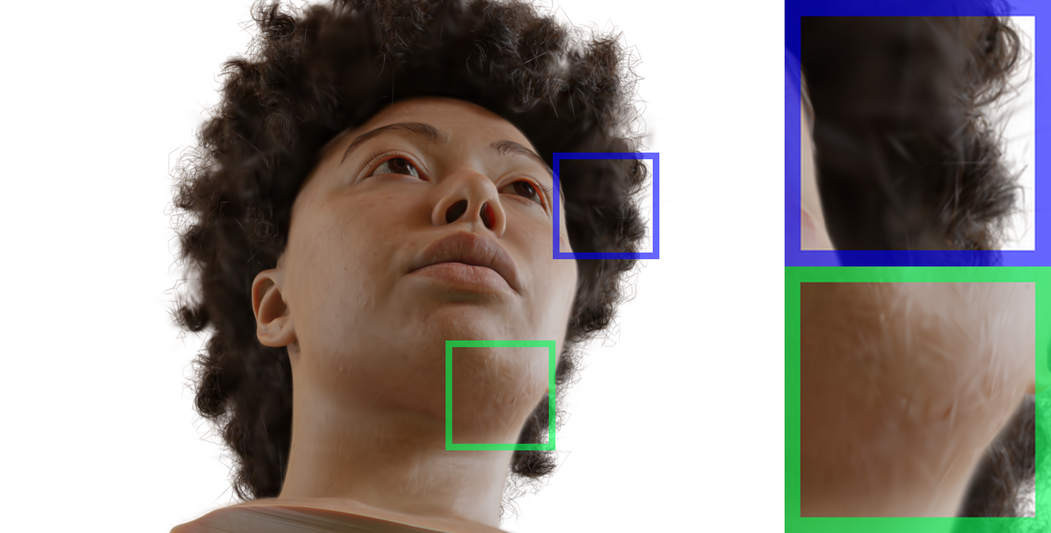
\includegraphics[width=\linewidth]{images/closeup/khady_3dgs_22_detail.png}
  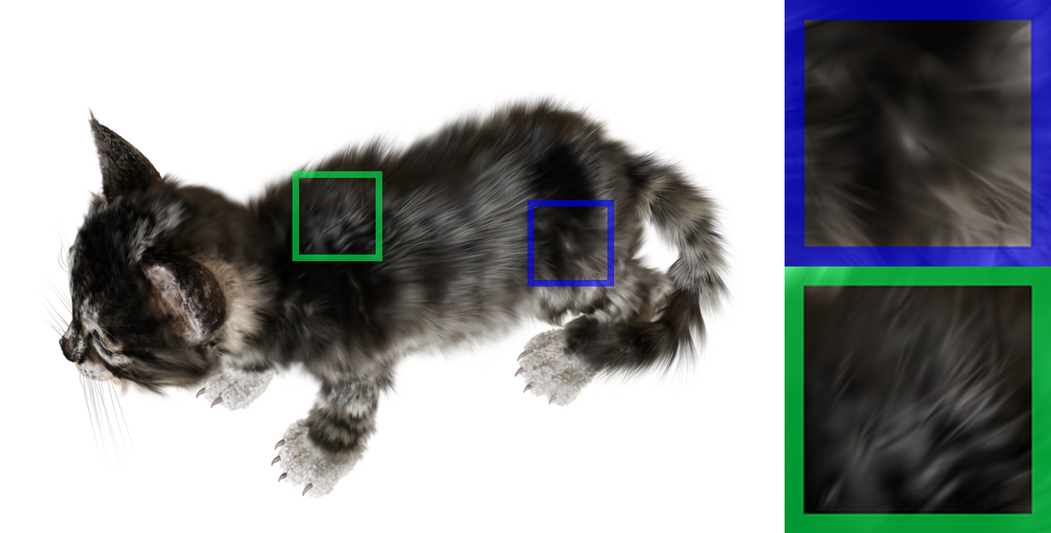
\includegraphics[width=\linewidth]{images/closeup/kitten_3dgs_67_detail.png}
  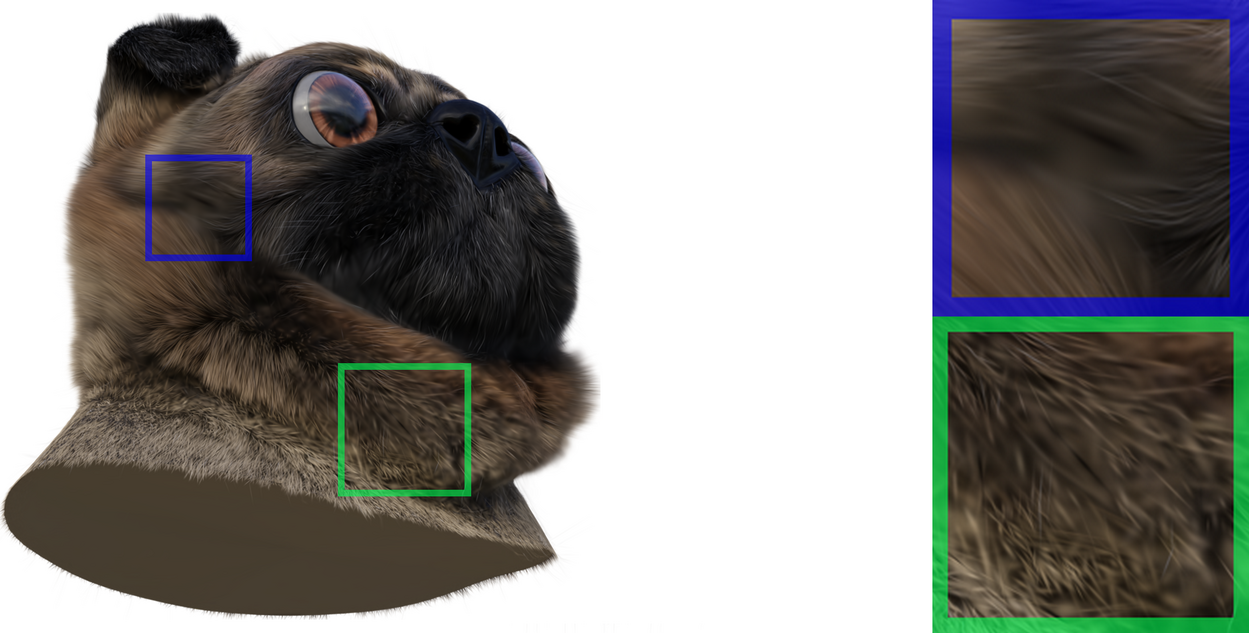
\includegraphics[width=\linewidth]{images/closeup/pug_3dgs_25_detail.png}
  \caption{3DGS~\cite{kerbl3Dgaussians}}
  \end{subfigure}
  %
  \hfill
  %
  \begin{subfigure}{0.31\linewidth}
  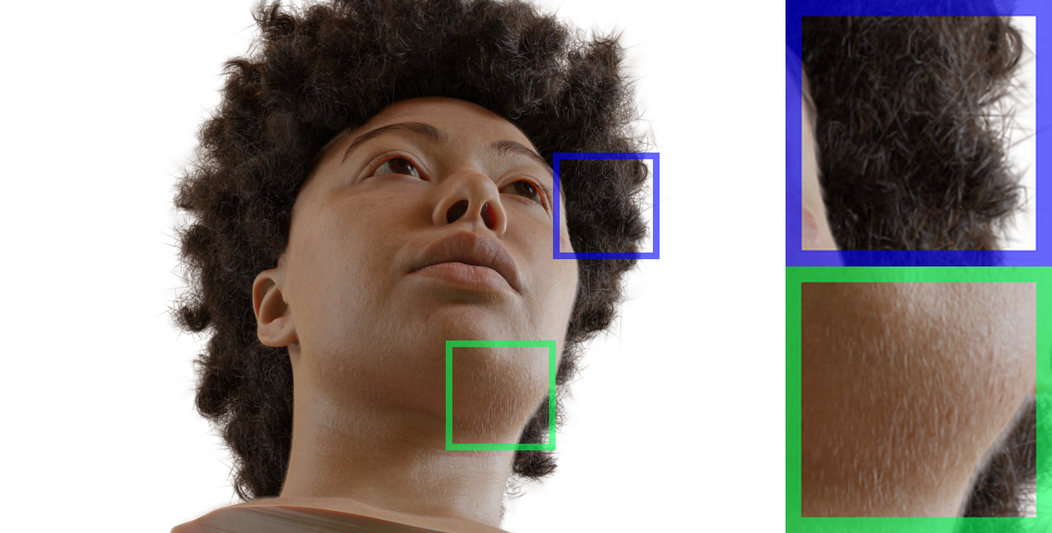
\includegraphics[width=\linewidth]{images/closeup/khady_rgb_22_detail.png}
  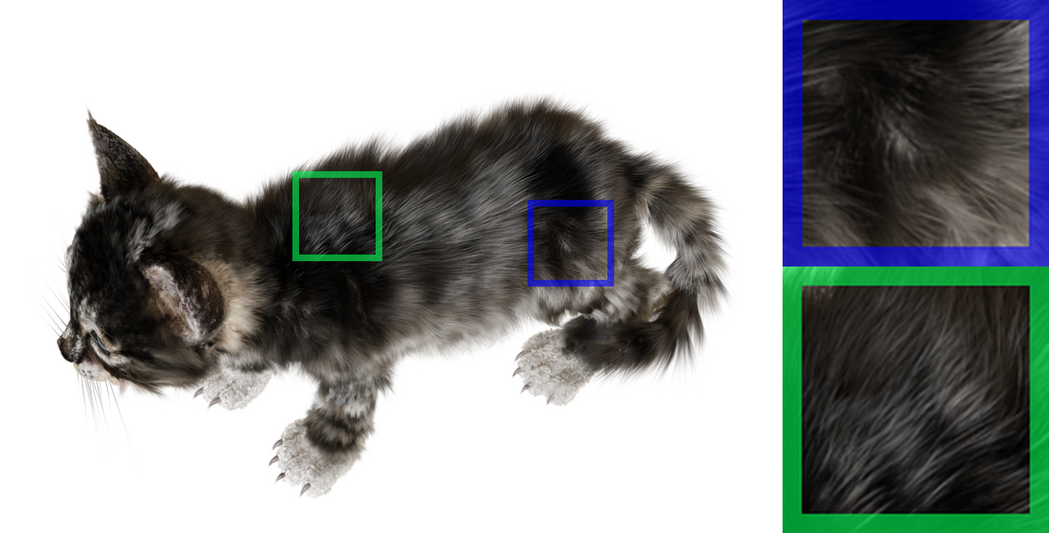
\includegraphics[width=\linewidth]{images/closeup/kitten_rgb_67_detail.png}
  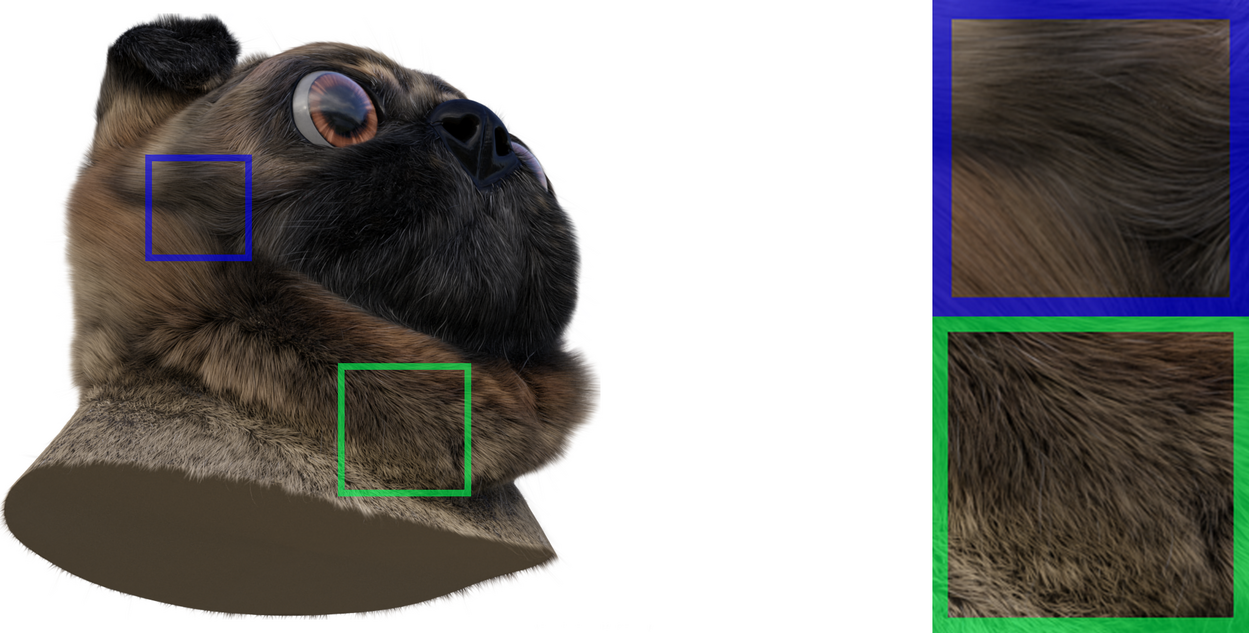
\includegraphics[width=\linewidth]{images/closeup/pug_rgb_25_detail.png}
  \caption*{Frosting (Ours)}
  \end{subfigure}
  %
  \vspace{-0.3cm}
  \caption{
  \textbf{Close-up views of fuzzy materials from the Shelly dataset~\cite{wang-siggraphasia2023-adaptive-shells} reconstructed with vanilla Gaussian Splatting~\cite{kerbl3Dgaussians}~(center) and Frosting~(right).}
  }
  \label{fig:fuzzy-material-closeup}
\end{figure}